% Plantilla para un Trabajo Fin de Grado de la Universidad de Granada,
% adaptada para el Doble Grado en Ingeniería Informática y Matemáticas.
%
%  Autor: Mario Román.
%  Licencia: GNU GPLv2.
%
% Esta plantilla es una adaptación al castellano de la plantilla
% classicthesis de André Miede, que puede obtenerse en:
%  https://ctan.org/tex-archive/macros/latex/contrib/classicthesis?lang=en
% La plantilla original se licencia en GNU GPLv2.
%
% Esta plantilla usa símbolos de la Universidad de Granada sujetos a la normativa
% de identidad visual corporativa, que puede encontrarse en:
% http://secretariageneral.ugr.es/pages/ivc/normativa
%
% La compilación se realiza con las siguientes instrucciones:
%   pdflatex --shell-escape main.tex
%   bibtex main
%   pdflatex --shell-escape main.tex
%   pdflatex --shell-escape main.tex

% Opciones del tipo de documento
\documentclass[twoside,openright,titlepage,numbers=noenddot,openany,headinclude,footinclude=true,
cleardoublepage=empty,abstractoff,BCOR=5mm,paper=a4,fontsize=12pt,main=spanish]{scrreprt}

% Paquetes de latex que se cargan al inicio. Cubren la entrada de
% texto, gráficos, código fuente y símbolofs.
\usepackage[utf8]{inputenc}
\usepackage[T1]{fontenc}
\usepackage{fixltx2e}
\usepackage{graphicx} % Inclusión de imágenes.
\usepackage{grffile}  % Distintos formatos para imágenes.
\usepackage{longtable} % Tablas multipágina.
\usepackage{wrapfig} % Coloca texto alrededor de una figura.
\usepackage{rotating}
\usepackage[normalem]{ulem}
\usepackage{amsmath}
\usepackage{dsfont}
\usepackage{textcomp}
\usepackage{amssymb}
\usepackage{capt-of}
\usepackage[colorlinks=true]{hyperref}
\usepackage{tikz} % Diagramas conmutativos.
\usepackage{minted} % Código fuente.
\usepackage[T1]{fontenc}
\usepackage[numbers]{natbib}

% PAQUETE MIO

\usepackage{float}

% Plantilla classicthesis
\usepackage[beramono,eulerchapternumbers,linedheaders,parts,a5paper,dottedtoc,
manychapters,pdfspacing]{classicthesis}

% Geometría y espaciado de párrafos.
\setcounter{secnumdepth}{0}
\usepackage{enumitem}
\setitemize{noitemsep,topsep=0pt,parsep=0pt,partopsep=0pt}
\setlist[enumerate]{topsep=0pt,itemsep=-1ex,partopsep=1ex,parsep=1ex}
\usepackage[top=1in, bottom=1.5in, left=1in, right=1in]{geometry}
\setlength\itemsep{0em}
\setlength{\parindent}{0pt}
\usepackage{parskip}

% Profundidad de la tabla de contenidos.
\setcounter{secnumdepth}{3}

% Usa el paquete minted para mostrar trozos de código.
% Pueden seleccionarse el lenguaje apropiado y el estilo del código.
\usepackage{minted}
\usemintedstyle{colorful}
\setminted{fontsize=\small}
\setminted[haskell]{linenos=false,fontsize=\small}
\renewcommand{\theFancyVerbLine}{\sffamily\textcolor[rgb]{0.5,0.5,1.0}{\oldstylenums{\arabic{FancyVerbLine}}}}

% Path para las imágenes
\graphicspath{{figures/}}

% Archivos de configuración.
%------------------------
% Bibliotecas para matemáticas de latex
%------------------------
\usepackage{amsthm}
\usepackage{amsmath}
\usepackage{tikz}
\usepackage{tikz-cd}
\usetikzlibrary{shapes,fit}
\usepackage{bussproofs}
\EnableBpAbbreviations{}
\usepackage{mathtools}
\usepackage{scalerel}
\usepackage{stmaryrd}

%------------------------
% Estilos para los teoremas
%------------------------
\theoremstyle{plain}
\newtheorem{theorem}{Teorema}
\newtheorem{proposition}{Proposición}
\newtheorem{lemma}{Lema}
\newtheorem{corollary}{Corolario}

\theoremstyle{definition}
\newtheorem{definition}{Definición}
\newtheorem{postulate}{Postulado}
\newtheorem*{postulate 3'}{Postulate 3'}
\newtheorem*{postulate 2'}{Projective Measurement}


% Comento estas lineas originales intentando que diga dem
%\renewenvironment{proof}{{\bfseries Proof.}}{\qed}

% Change the proof style so it's in English and add \qed at the end.
%\renewenvironment{proof}{{\bfseries Proof.}}{\qed}

% Añadido por mi intentando que pone "Demostración" y no "Proof"
\renewenvironment{proof}{{\bfseries Demostración.}}{\qed}
\renewenvironment{proof}{{\bfseries Demostración.}}{\qed}
% hasta aqui

\theoremstyle{remark}
\newtheorem{remark}{Remark}
\newtheorem{exampleth}{Ejemplo}

\begingroup\makeatletter\@for\theoremstyle:=definition,remark,plain\do{\expandafter\g@addto@macro\csname th@\theoremstyle\endcsname{\addtolength\thm@preskip\parskip}}\endgroup

%------------------------
% Macros
% ------------------------

\newcommand*{\C}{\mathds{C}}
\newcommand*{\ra}{\rangle}
\newcommand*{\la}{\langle}

% Para poner sonrisa sobre puntos suspensivos. Uso: \overplace{n}{\dotsc}
\newcommand{\overplace}[2]{%
	\overset{\substack{#1\\\smile}}{#2}%
}  % En macros.tex se almacenan las opciones y comandos para escribir matemáticas.
% ****************************************************************************************************
% classicthesis-config.tex 
% formerly known as loadpackages.sty, classicthesis-ldpkg.sty, and classicthesis-preamble.sty 
% Use it at the beginning of your ClassicThesis.tex, or as a LaTeX Preamble 
% in your ClassicThesis.{tex,lyx} with % ****************************************************************************************************
% classicthesis-config.tex 
% formerly known as loadpackages.sty, classicthesis-ldpkg.sty, and classicthesis-preamble.sty 
% Use it at the beginning of your ClassicThesis.tex, or as a LaTeX Preamble 
% in your ClassicThesis.{tex,lyx} with % ****************************************************************************************************
% classicthesis-config.tex 
% formerly known as loadpackages.sty, classicthesis-ldpkg.sty, and classicthesis-preamble.sty 
% Use it at the beginning of your ClassicThesis.tex, or as a LaTeX Preamble 
% in your ClassicThesis.{tex,lyx} with \input{classicthesis-config}
% ****************************************************************************************************  
% If you like the classicthesis, then I would appreciate a postcard. 
% My address can be found in the file ClassicThesis.pdf. A collection 
% of the postcards I received so far is available online at 
% http://postcards.miede.de
% ****************************************************************************************************


% ****************************************************************************************************
% 0. Set the encoding of your files. UTF-8 is the only sensible encoding nowadays. If you can't read
% äöüßáéçèê∂åëæƒÏ€ then change the encoding setting in your editor, not the line below. If your editor
% does not support utf8 use another editor!
% ****************************************************************************************************
\PassOptionsToPackage{utf8x}{inputenc}
	\usepackage{inputenc}

% ****************************************************************************************************
% 1. Configure classicthesis for your needs here, e.g., remove "drafting" below 
% in order to deactivate the time-stamp on the pages
% ****************************************************************************************************
\PassOptionsToPackage{eulerchapternumbers,listings,drafting,%
		pdfspacing,%floatperchapter,%linedheaders,%
                subfig,beramono,eulermath,parts,dottedtoc}{classicthesis}                                        
% ********************************************************************
% Available options for classicthesis.sty 
% (see ClassicThesis.pdf for more information):
% drafting
% parts nochapters linedheaders
% eulerchapternumbers beramono eulermath pdfspacing minionprospacing
% tocaligned dottedtoc manychapters
% listings floatperchapter subfig
% ********************************************************************

% ****************************************************************************************************
% 2. Personal data and user ad-hoc commands
% ****************************************************************************************************
\newcommand{\myTitle}{Practica 3\xspace}
\newcommand{\mySubtitle}{An Homage to The Elements of Typographic Style\xspace}
\newcommand{\myDegree}{Doktor-Ingenieur (Dr.-Ing.)\xspace}
\newcommand{\myName}{André Miede\xspace}
\newcommand{\myProf}{Put name here\xspace}
\newcommand{\myOtherProf}{Put name here\xspace}
\newcommand{\mySupervisor}{Put name here\xspace}
\newcommand{\myFaculty}{Put data here\xspace}
\newcommand{\myDepartment}{Put data here\xspace}
\newcommand{\myUni}{Put data here\xspace}
\newcommand{\myLocation}{Saarbrücken\xspace}
\newcommand{\myTime}{September 2015\xspace}
%\newcommand{\myVersion}{version 4.2\xspace}

% ********************************************************************
% Setup, finetuning, and useful commands
% ********************************************************************
\newcounter{dummy} % necessary for correct hyperlinks (to index, bib, etc.)
\newlength{\abcd} % for ab..z string length calculation
\providecommand{\mLyX}{L\kern-.1667em\lower.25em\hbox{Y}\kern-.125emX\@}
\newcommand{\ie}{i.\,e.}
\newcommand{\Ie}{I.\,e.}
\newcommand{\eg}{e.\,g.}
\newcommand{\Eg}{E.\,g.} 
% ****************************************************************************************************


% ****************************************************************************************************
% 3. Loading some handy packages
% ****************************************************************************************************
% ******************************************************************** 
% Packages with options that might require adjustments
% ******************************************************************** 
%\PassOptionsToPackage{ngerman,american}{babel}   % change this to your language(s)
% Spanish languages need extra options in order to work with this template
% \PassOptionsToPackage{es-lcroman,spanish}{babel}
\usepackage[main=spanish]{babel}

%\usepackage{csquotes}
% \PassOptionsToPackage{%
%     %backend=biber, %instead of bibtex
% 	backend=bibtex8,bibencoding=ascii,%
% 	language=auto,%
% 	style=alpha,%
%     %style=authoryear-comp, % Author 1999, 2010
%     %bibstyle=authoryear,dashed=false, % dashed: substitute rep. author with ---
%     sorting=nyt, % name, year, title
%     maxbibnames=10, % default: 3, et al.
%     %backref=true,%
%     natbib=true % natbib compatibility mode (\citep and \citet still work)
% }{biblatex}
%     \usepackage{biblatex}

% \PassOptionsToPackage{fleqn}{amsmath}       % math environments and more by the AMS 
%     \usepackage{amsmath}

% ******************************************************************** 
% General useful packages
% ******************************************************************** 
\PassOptionsToPackage{T1}{fontenc} % T2A for cyrillics
    \usepackage{fontenc}     
\usepackage{textcomp} % fix warning with missing font shapes
\usepackage{scrhack} % fix warnings when using KOMA with listings package          
\usepackage{xspace} % to get the spacing after macros right  
\usepackage{mparhack} % get marginpar right
\usepackage{fixltx2e} % fixes some LaTeX stuff --> since 2015 in the LaTeX kernel (see below)
%\usepackage[latest]{latexrelease} % will be used once available in more distributions (ISSUE #107)
\PassOptionsToPackage{printonlyused,smaller}{acronym} 
    \usepackage{acronym} % nice macros for handling all acronyms in the thesis
    %\renewcommand{\bflabel}[1]{{#1}\hfill} % fix the list of acronyms --> no longer working
    %\renewcommand*{\acsfont}[1]{\textsc{#1}} 
    \renewcommand*{\aclabelfont}[1]{\acsfont{#1}}
% ****************************************************************************************************


% ****************************************************************************************************
% 4. Setup floats: tables, (sub)figures, and captions
% ****************************************************************************************************
\usepackage{tabularx} % better tables
    \setlength{\extrarowheight}{3pt} % increase table row height
\newcommand{\tableheadline}[1]{\multicolumn{1}{c}{\spacedlowsmallcaps{#1}}}
\newcommand{\myfloatalign}{\centering} % to be used with each float for alignment
\usepackage{caption}
% Thanks to cgnieder and Claus Lahiri
% http://tex.stackexchange.com/questions/69349/spacedlowsmallcaps-in-caption-label
% [REMOVED DUE TO OTHER PROBLEMS, SEE ISSUE #82]    
%\DeclareCaptionLabelFormat{smallcaps}{\bothIfFirst{#1}{~}\MakeTextLowercase{\textsc{#2}}}
%\captionsetup{font=small,labelformat=smallcaps} % format=hang,
\captionsetup{font=small} % format=hang,
\usepackage{subfig}  
% ****************************************************************************************************


% ****************************************************************************************************
% 5. Setup code listings
% ****************************************************************************************************
% \usepackage{listings} 
% %\lstset{emph={trueIndex,root},emphstyle=\color{BlueViolet}}%\underbar} % for special keywords
% \lstset{language={Haskell},morekeywords={PassOptionsToPackage,selectlanguage},keywordstyle=\color{RoyalBlue},basicstyle=\small\ttfamily,commentstyle=\color{Green}\ttfamily,stringstyle=\rmfamily,numbers=none,numberstyle=\scriptsize,stepnumber=5,numbersep=8pt,showstringspaces=false,breaklines=true,belowcaptionskip=.75\baselineskip} 
% ****************************************************************************************************             


% ****************************************************************************************************
% 6. PDFLaTeX, hyperreferences and citation backreferences
% ****************************************************************************************************
% ********************************************************************
% Using PDFLaTeX
% ********************************************************************
\PassOptionsToPackage{pdftex,hyperfootnotes=false,pdfpagelabels}{hyperref}
    \usepackage{hyperref}  % backref linktocpage pagebackref
\pdfcompresslevel=9
\pdfadjustspacing=1 
\PassOptionsToPackage{pdftex}{graphicx}
    \usepackage{graphicx} 
 

% ********************************************************************
% Hyperreferences
% ********************************************************************
\hypersetup{%
    %draft, % = no hyperlinking at all (useful in b/w printouts)
    colorlinks=true, linktocpage=true, pdfstartpage=3, pdfstartview=FitV,%
    % uncomment the following line if you want to have black links (e.g., for printing)
    %colorlinks=false, linktocpage=false, pdfstartpage=3, pdfstartview=FitV, pdfborder={0 0 0},%
    breaklinks=true, pdfpagemode=UseNone, pageanchor=true, pdfpagemode=UseOutlines,%
    plainpages=false, bookmarksnumbered, bookmarksopen=true, bookmarksopenlevel=1,%
    hypertexnames=true, pdfhighlight=/O,%nesting=true,%frenchlinks,%
    urlcolor=webbrown, linkcolor=RoyalBlue, citecolor=webgreen, %pagecolor=RoyalBlue,%
    %urlcolor=Black, linkcolor=Black, citecolor=Black, %pagecolor=Black,%
    pdftitle={\myTitle},%
    pdfauthor={\textcopyright\ \myName, \myUni, \myFaculty},%
    pdfsubject={},%
    pdfkeywords={},%
    pdfcreator={pdfLaTeX},%
    pdfproducer={LaTeX with hyperref and classicthesis}%
}   

% ********************************************************************
% Setup autoreferences
% ********************************************************************
% There are some issues regarding autorefnames
% http://www.ureader.de/msg/136221647.aspx
% http://www.tex.ac.uk/cgi-bin/texfaq2html?label=latexwords
% you have to redefine the makros for the 
% language you use, e.g., american, ngerman
% (as chosen when loading babel/AtBeginDocument)
% ********************************************************************
\makeatletter
\@ifpackageloaded{babel}%
    {%
       \addto\extrasamerican{%
			\renewcommand*{\figureautorefname}{Figure}%
			\renewcommand*{\tableautorefname}{Table}%
			\renewcommand*{\partautorefname}{Part}%
			\renewcommand*{\chapterautorefname}{Chapter}%
			\renewcommand*{\sectionautorefname}{Section}%
			\renewcommand*{\subsectionautorefname}{Section}%
			\renewcommand*{\subsubsectionautorefname}{Section}%     
                }%
       \addto\extrasngerman{% 
			\renewcommand*{\paragraphautorefname}{Absatz}%
			\renewcommand*{\subparagraphautorefname}{Unterabsatz}%
			\renewcommand*{\footnoteautorefname}{Fu\"snote}%
			\renewcommand*{\FancyVerbLineautorefname}{Zeile}%
			\renewcommand*{\theoremautorefname}{Theorem}%
			\renewcommand*{\appendixautorefname}{Anhang}%
			\renewcommand*{\equationautorefname}{Gleichung}%        
			\renewcommand*{\itemautorefname}{Punkt}%
                }%  
            % Fix to getting autorefs for subfigures right (thanks to Belinda Vogt for changing the definition)
            \providecommand{\subfigureautorefname}{\figureautorefname}%             
    }{\relax}
\makeatother


% ****************************************************************************************************
% 7. Last calls before the bar closes
% ****************************************************************************************************
% ********************************************************************
% Development Stuff
% ********************************************************************
\listfiles
%\PassOptionsToPackage{l2tabu,orthodox,abort}{nag}
%   \usepackage{nag}
%\PassOptionsToPackage{warning, all}{onlyamsmath}
%   \usepackage{onlyamsmath}

% ********************************************************************
% Last, but not least...
% ********************************************************************
\usepackage{classicthesis} 
% ****************************************************************************************************


% ****************************************************************************************************
% 8. Further adjustments (experimental)
% ****************************************************************************************************
% ********************************************************************
% Changing the text area
% ********************************************************************
%\linespread{1.05} % a bit more for Palatino
%\areaset[current]{312pt}{761pt} % 686 (factor 2.2) + 33 head + 42 head \the\footskip
%\setlength{\marginparwidth}{7em}%
%\setlength{\marginparsep}{2em}%

% ********************************************************************
% Using different fonts
% ********************************************************************
%\usepackage[oldstylenums]{kpfonts} % oldstyle notextcomp
%\usepackage[osf]{libertine}
%\usepackage[light,condensed,math]{iwona}
%\renewcommand{\sfdefault}{iwona}
%\usepackage{lmodern} % <-- no osf support :-(
%\usepackage{cfr-lm} % 
%\usepackage[urw-garamond]{mathdesign} <-- no osf support :-(
%\usepackage[default,osfigures]{opensans} % scale=0.95 
%\usepackage[sfdefault]{FiraSans}
% ****************************************************************************************************

% ****************************************************************************************************  
% If you like the classicthesis, then I would appreciate a postcard. 
% My address can be found in the file ClassicThesis.pdf. A collection 
% of the postcards I received so far is available online at 
% http://postcards.miede.de
% ****************************************************************************************************


% ****************************************************************************************************
% 0. Set the encoding of your files. UTF-8 is the only sensible encoding nowadays. If you can't read
% äöüßáéçèê∂åëæƒÏ€ then change the encoding setting in your editor, not the line below. If your editor
% does not support utf8 use another editor!
% ****************************************************************************************************
\PassOptionsToPackage{utf8x}{inputenc}
	\usepackage{inputenc}

% ****************************************************************************************************
% 1. Configure classicthesis for your needs here, e.g., remove "drafting" below 
% in order to deactivate the time-stamp on the pages
% ****************************************************************************************************
\PassOptionsToPackage{eulerchapternumbers,listings,drafting,%
		pdfspacing,%floatperchapter,%linedheaders,%
                subfig,beramono,eulermath,parts,dottedtoc}{classicthesis}                                        
% ********************************************************************
% Available options for classicthesis.sty 
% (see ClassicThesis.pdf for more information):
% drafting
% parts nochapters linedheaders
% eulerchapternumbers beramono eulermath pdfspacing minionprospacing
% tocaligned dottedtoc manychapters
% listings floatperchapter subfig
% ********************************************************************

% ****************************************************************************************************
% 2. Personal data and user ad-hoc commands
% ****************************************************************************************************
\newcommand{\myTitle}{Practica 3\xspace}
\newcommand{\mySubtitle}{An Homage to The Elements of Typographic Style\xspace}
\newcommand{\myDegree}{Doktor-Ingenieur (Dr.-Ing.)\xspace}
\newcommand{\myName}{André Miede\xspace}
\newcommand{\myProf}{Put name here\xspace}
\newcommand{\myOtherProf}{Put name here\xspace}
\newcommand{\mySupervisor}{Put name here\xspace}
\newcommand{\myFaculty}{Put data here\xspace}
\newcommand{\myDepartment}{Put data here\xspace}
\newcommand{\myUni}{Put data here\xspace}
\newcommand{\myLocation}{Saarbrücken\xspace}
\newcommand{\myTime}{September 2015\xspace}
%\newcommand{\myVersion}{version 4.2\xspace}

% ********************************************************************
% Setup, finetuning, and useful commands
% ********************************************************************
\newcounter{dummy} % necessary for correct hyperlinks (to index, bib, etc.)
\newlength{\abcd} % for ab..z string length calculation
\providecommand{\mLyX}{L\kern-.1667em\lower.25em\hbox{Y}\kern-.125emX\@}
\newcommand{\ie}{i.\,e.}
\newcommand{\Ie}{I.\,e.}
\newcommand{\eg}{e.\,g.}
\newcommand{\Eg}{E.\,g.} 
% ****************************************************************************************************


% ****************************************************************************************************
% 3. Loading some handy packages
% ****************************************************************************************************
% ******************************************************************** 
% Packages with options that might require adjustments
% ******************************************************************** 
%\PassOptionsToPackage{ngerman,american}{babel}   % change this to your language(s)
% Spanish languages need extra options in order to work with this template
% \PassOptionsToPackage{es-lcroman,spanish}{babel}
\usepackage[main=spanish]{babel}

%\usepackage{csquotes}
% \PassOptionsToPackage{%
%     %backend=biber, %instead of bibtex
% 	backend=bibtex8,bibencoding=ascii,%
% 	language=auto,%
% 	style=alpha,%
%     %style=authoryear-comp, % Author 1999, 2010
%     %bibstyle=authoryear,dashed=false, % dashed: substitute rep. author with ---
%     sorting=nyt, % name, year, title
%     maxbibnames=10, % default: 3, et al.
%     %backref=true,%
%     natbib=true % natbib compatibility mode (\citep and \citet still work)
% }{biblatex}
%     \usepackage{biblatex}

% \PassOptionsToPackage{fleqn}{amsmath}       % math environments and more by the AMS 
%     \usepackage{amsmath}

% ******************************************************************** 
% General useful packages
% ******************************************************************** 
\PassOptionsToPackage{T1}{fontenc} % T2A for cyrillics
    \usepackage{fontenc}     
\usepackage{textcomp} % fix warning with missing font shapes
\usepackage{scrhack} % fix warnings when using KOMA with listings package          
\usepackage{xspace} % to get the spacing after macros right  
\usepackage{mparhack} % get marginpar right
\usepackage{fixltx2e} % fixes some LaTeX stuff --> since 2015 in the LaTeX kernel (see below)
%\usepackage[latest]{latexrelease} % will be used once available in more distributions (ISSUE #107)
\PassOptionsToPackage{printonlyused,smaller}{acronym} 
    \usepackage{acronym} % nice macros for handling all acronyms in the thesis
    %\renewcommand{\bflabel}[1]{{#1}\hfill} % fix the list of acronyms --> no longer working
    %\renewcommand*{\acsfont}[1]{\textsc{#1}} 
    \renewcommand*{\aclabelfont}[1]{\acsfont{#1}}
% ****************************************************************************************************


% ****************************************************************************************************
% 4. Setup floats: tables, (sub)figures, and captions
% ****************************************************************************************************
\usepackage{tabularx} % better tables
    \setlength{\extrarowheight}{3pt} % increase table row height
\newcommand{\tableheadline}[1]{\multicolumn{1}{c}{\spacedlowsmallcaps{#1}}}
\newcommand{\myfloatalign}{\centering} % to be used with each float for alignment
\usepackage{caption}
% Thanks to cgnieder and Claus Lahiri
% http://tex.stackexchange.com/questions/69349/spacedlowsmallcaps-in-caption-label
% [REMOVED DUE TO OTHER PROBLEMS, SEE ISSUE #82]    
%\DeclareCaptionLabelFormat{smallcaps}{\bothIfFirst{#1}{~}\MakeTextLowercase{\textsc{#2}}}
%\captionsetup{font=small,labelformat=smallcaps} % format=hang,
\captionsetup{font=small} % format=hang,
\usepackage{subfig}  
% ****************************************************************************************************


% ****************************************************************************************************
% 5. Setup code listings
% ****************************************************************************************************
% \usepackage{listings} 
% %\lstset{emph={trueIndex,root},emphstyle=\color{BlueViolet}}%\underbar} % for special keywords
% \lstset{language={Haskell},morekeywords={PassOptionsToPackage,selectlanguage},keywordstyle=\color{RoyalBlue},basicstyle=\small\ttfamily,commentstyle=\color{Green}\ttfamily,stringstyle=\rmfamily,numbers=none,numberstyle=\scriptsize,stepnumber=5,numbersep=8pt,showstringspaces=false,breaklines=true,belowcaptionskip=.75\baselineskip} 
% ****************************************************************************************************             


% ****************************************************************************************************
% 6. PDFLaTeX, hyperreferences and citation backreferences
% ****************************************************************************************************
% ********************************************************************
% Using PDFLaTeX
% ********************************************************************
\PassOptionsToPackage{pdftex,hyperfootnotes=false,pdfpagelabels}{hyperref}
    \usepackage{hyperref}  % backref linktocpage pagebackref
\pdfcompresslevel=9
\pdfadjustspacing=1 
\PassOptionsToPackage{pdftex}{graphicx}
    \usepackage{graphicx} 
 

% ********************************************************************
% Hyperreferences
% ********************************************************************
\hypersetup{%
    %draft, % = no hyperlinking at all (useful in b/w printouts)
    colorlinks=true, linktocpage=true, pdfstartpage=3, pdfstartview=FitV,%
    % uncomment the following line if you want to have black links (e.g., for printing)
    %colorlinks=false, linktocpage=false, pdfstartpage=3, pdfstartview=FitV, pdfborder={0 0 0},%
    breaklinks=true, pdfpagemode=UseNone, pageanchor=true, pdfpagemode=UseOutlines,%
    plainpages=false, bookmarksnumbered, bookmarksopen=true, bookmarksopenlevel=1,%
    hypertexnames=true, pdfhighlight=/O,%nesting=true,%frenchlinks,%
    urlcolor=webbrown, linkcolor=RoyalBlue, citecolor=webgreen, %pagecolor=RoyalBlue,%
    %urlcolor=Black, linkcolor=Black, citecolor=Black, %pagecolor=Black,%
    pdftitle={\myTitle},%
    pdfauthor={\textcopyright\ \myName, \myUni, \myFaculty},%
    pdfsubject={},%
    pdfkeywords={},%
    pdfcreator={pdfLaTeX},%
    pdfproducer={LaTeX with hyperref and classicthesis}%
}   

% ********************************************************************
% Setup autoreferences
% ********************************************************************
% There are some issues regarding autorefnames
% http://www.ureader.de/msg/136221647.aspx
% http://www.tex.ac.uk/cgi-bin/texfaq2html?label=latexwords
% you have to redefine the makros for the 
% language you use, e.g., american, ngerman
% (as chosen when loading babel/AtBeginDocument)
% ********************************************************************
\makeatletter
\@ifpackageloaded{babel}%
    {%
       \addto\extrasamerican{%
			\renewcommand*{\figureautorefname}{Figure}%
			\renewcommand*{\tableautorefname}{Table}%
			\renewcommand*{\partautorefname}{Part}%
			\renewcommand*{\chapterautorefname}{Chapter}%
			\renewcommand*{\sectionautorefname}{Section}%
			\renewcommand*{\subsectionautorefname}{Section}%
			\renewcommand*{\subsubsectionautorefname}{Section}%     
                }%
       \addto\extrasngerman{% 
			\renewcommand*{\paragraphautorefname}{Absatz}%
			\renewcommand*{\subparagraphautorefname}{Unterabsatz}%
			\renewcommand*{\footnoteautorefname}{Fu\"snote}%
			\renewcommand*{\FancyVerbLineautorefname}{Zeile}%
			\renewcommand*{\theoremautorefname}{Theorem}%
			\renewcommand*{\appendixautorefname}{Anhang}%
			\renewcommand*{\equationautorefname}{Gleichung}%        
			\renewcommand*{\itemautorefname}{Punkt}%
                }%  
            % Fix to getting autorefs for subfigures right (thanks to Belinda Vogt for changing the definition)
            \providecommand{\subfigureautorefname}{\figureautorefname}%             
    }{\relax}
\makeatother


% ****************************************************************************************************
% 7. Last calls before the bar closes
% ****************************************************************************************************
% ********************************************************************
% Development Stuff
% ********************************************************************
\listfiles
%\PassOptionsToPackage{l2tabu,orthodox,abort}{nag}
%   \usepackage{nag}
%\PassOptionsToPackage{warning, all}{onlyamsmath}
%   \usepackage{onlyamsmath}

% ********************************************************************
% Last, but not least...
% ********************************************************************
\usepackage{classicthesis} 
% ****************************************************************************************************


% ****************************************************************************************************
% 8. Further adjustments (experimental)
% ****************************************************************************************************
% ********************************************************************
% Changing the text area
% ********************************************************************
%\linespread{1.05} % a bit more for Palatino
%\areaset[current]{312pt}{761pt} % 686 (factor 2.2) + 33 head + 42 head \the\footskip
%\setlength{\marginparwidth}{7em}%
%\setlength{\marginparsep}{2em}%

% ********************************************************************
% Using different fonts
% ********************************************************************
%\usepackage[oldstylenums]{kpfonts} % oldstyle notextcomp
%\usepackage[osf]{libertine}
%\usepackage[light,condensed,math]{iwona}
%\renewcommand{\sfdefault}{iwona}
%\usepackage{lmodern} % <-- no osf support :-(
%\usepackage{cfr-lm} % 
%\usepackage[urw-garamond]{mathdesign} <-- no osf support :-(
%\usepackage[default,osfigures]{opensans} % scale=0.95 
%\usepackage[sfdefault]{FiraSans}
% ****************************************************************************************************

% ****************************************************************************************************  
% If you like the classicthesis, then I would appreciate a postcard. 
% My address can be found in the file ClassicThesis.pdf. A collection 
% of the postcards I received so far is available online at 
% http://postcards.miede.de
% ****************************************************************************************************


% ****************************************************************************************************
% 0. Set the encoding of your files. UTF-8 is the only sensible encoding nowadays. If you can't read
% äöüßáéçèê∂åëæƒÏ€ then change the encoding setting in your editor, not the line below. If your editor
% does not support utf8 use another editor!
% ****************************************************************************************************
\PassOptionsToPackage{utf8x}{inputenc}
	\usepackage{inputenc}

% ****************************************************************************************************
% 1. Configure classicthesis for your needs here, e.g., remove "drafting" below 
% in order to deactivate the time-stamp on the pages
% ****************************************************************************************************
\PassOptionsToPackage{eulerchapternumbers,listings,drafting,%
		pdfspacing,%floatperchapter,%linedheaders,%
                subfig,beramono,eulermath,parts,dottedtoc}{classicthesis}                                        
% ********************************************************************
% Available options for classicthesis.sty 
% (see ClassicThesis.pdf for more information):
% drafting
% parts nochapters linedheaders
% eulerchapternumbers beramono eulermath pdfspacing minionprospacing
% tocaligned dottedtoc manychapters
% listings floatperchapter subfig
% ********************************************************************

% ****************************************************************************************************
% 2. Personal data and user ad-hoc commands
% ****************************************************************************************************
\newcommand{\myTitle}{Practica 3\xspace}
\newcommand{\mySubtitle}{An Homage to The Elements of Typographic Style\xspace}
\newcommand{\myDegree}{Doktor-Ingenieur (Dr.-Ing.)\xspace}
\newcommand{\myName}{André Miede\xspace}
\newcommand{\myProf}{Put name here\xspace}
\newcommand{\myOtherProf}{Put name here\xspace}
\newcommand{\mySupervisor}{Put name here\xspace}
\newcommand{\myFaculty}{Put data here\xspace}
\newcommand{\myDepartment}{Put data here\xspace}
\newcommand{\myUni}{Put data here\xspace}
\newcommand{\myLocation}{Saarbrücken\xspace}
\newcommand{\myTime}{September 2015\xspace}
%\newcommand{\myVersion}{version 4.2\xspace}

% ********************************************************************
% Setup, finetuning, and useful commands
% ********************************************************************
\newcounter{dummy} % necessary for correct hyperlinks (to index, bib, etc.)
\newlength{\abcd} % for ab..z string length calculation
\providecommand{\mLyX}{L\kern-.1667em\lower.25em\hbox{Y}\kern-.125emX\@}
\newcommand{\ie}{i.\,e.}
\newcommand{\Ie}{I.\,e.}
\newcommand{\eg}{e.\,g.}
\newcommand{\Eg}{E.\,g.} 
% ****************************************************************************************************


% ****************************************************************************************************
% 3. Loading some handy packages
% ****************************************************************************************************
% ******************************************************************** 
% Packages with options that might require adjustments
% ******************************************************************** 
%\PassOptionsToPackage{ngerman,american}{babel}   % change this to your language(s)
% Spanish languages need extra options in order to work with this template
% \PassOptionsToPackage{es-lcroman,spanish}{babel}
\usepackage[main=spanish]{babel}

%\usepackage{csquotes}
% \PassOptionsToPackage{%
%     %backend=biber, %instead of bibtex
% 	backend=bibtex8,bibencoding=ascii,%
% 	language=auto,%
% 	style=alpha,%
%     %style=authoryear-comp, % Author 1999, 2010
%     %bibstyle=authoryear,dashed=false, % dashed: substitute rep. author with ---
%     sorting=nyt, % name, year, title
%     maxbibnames=10, % default: 3, et al.
%     %backref=true,%
%     natbib=true % natbib compatibility mode (\citep and \citet still work)
% }{biblatex}
%     \usepackage{biblatex}

% \PassOptionsToPackage{fleqn}{amsmath}       % math environments and more by the AMS 
%     \usepackage{amsmath}

% ******************************************************************** 
% General useful packages
% ******************************************************************** 
\PassOptionsToPackage{T1}{fontenc} % T2A for cyrillics
    \usepackage{fontenc}     
\usepackage{textcomp} % fix warning with missing font shapes
\usepackage{scrhack} % fix warnings when using KOMA with listings package          
\usepackage{xspace} % to get the spacing after macros right  
\usepackage{mparhack} % get marginpar right
\usepackage{fixltx2e} % fixes some LaTeX stuff --> since 2015 in the LaTeX kernel (see below)
%\usepackage[latest]{latexrelease} % will be used once available in more distributions (ISSUE #107)
\PassOptionsToPackage{printonlyused,smaller}{acronym} 
    \usepackage{acronym} % nice macros for handling all acronyms in the thesis
    %\renewcommand{\bflabel}[1]{{#1}\hfill} % fix the list of acronyms --> no longer working
    %\renewcommand*{\acsfont}[1]{\textsc{#1}} 
    \renewcommand*{\aclabelfont}[1]{\acsfont{#1}}
% ****************************************************************************************************


% ****************************************************************************************************
% 4. Setup floats: tables, (sub)figures, and captions
% ****************************************************************************************************
\usepackage{tabularx} % better tables
    \setlength{\extrarowheight}{3pt} % increase table row height
\newcommand{\tableheadline}[1]{\multicolumn{1}{c}{\spacedlowsmallcaps{#1}}}
\newcommand{\myfloatalign}{\centering} % to be used with each float for alignment
\usepackage{caption}
% Thanks to cgnieder and Claus Lahiri
% http://tex.stackexchange.com/questions/69349/spacedlowsmallcaps-in-caption-label
% [REMOVED DUE TO OTHER PROBLEMS, SEE ISSUE #82]    
%\DeclareCaptionLabelFormat{smallcaps}{\bothIfFirst{#1}{~}\MakeTextLowercase{\textsc{#2}}}
%\captionsetup{font=small,labelformat=smallcaps} % format=hang,
\captionsetup{font=small} % format=hang,
\usepackage{subfig}  
% ****************************************************************************************************


% ****************************************************************************************************
% 5. Setup code listings
% ****************************************************************************************************
% \usepackage{listings} 
% %\lstset{emph={trueIndex,root},emphstyle=\color{BlueViolet}}%\underbar} % for special keywords
% \lstset{language={Haskell},morekeywords={PassOptionsToPackage,selectlanguage},keywordstyle=\color{RoyalBlue},basicstyle=\small\ttfamily,commentstyle=\color{Green}\ttfamily,stringstyle=\rmfamily,numbers=none,numberstyle=\scriptsize,stepnumber=5,numbersep=8pt,showstringspaces=false,breaklines=true,belowcaptionskip=.75\baselineskip} 
% ****************************************************************************************************             


% ****************************************************************************************************
% 6. PDFLaTeX, hyperreferences and citation backreferences
% ****************************************************************************************************
% ********************************************************************
% Using PDFLaTeX
% ********************************************************************
\PassOptionsToPackage{pdftex,hyperfootnotes=false,pdfpagelabels}{hyperref}
    \usepackage{hyperref}  % backref linktocpage pagebackref
\pdfcompresslevel=9
\pdfadjustspacing=1 
\PassOptionsToPackage{pdftex}{graphicx}
    \usepackage{graphicx} 
 

% ********************************************************************
% Hyperreferences
% ********************************************************************
\hypersetup{%
    %draft, % = no hyperlinking at all (useful in b/w printouts)
    colorlinks=true, linktocpage=true, pdfstartpage=3, pdfstartview=FitV,%
    % uncomment the following line if you want to have black links (e.g., for printing)
    %colorlinks=false, linktocpage=false, pdfstartpage=3, pdfstartview=FitV, pdfborder={0 0 0},%
    breaklinks=true, pdfpagemode=UseNone, pageanchor=true, pdfpagemode=UseOutlines,%
    plainpages=false, bookmarksnumbered, bookmarksopen=true, bookmarksopenlevel=1,%
    hypertexnames=true, pdfhighlight=/O,%nesting=true,%frenchlinks,%
    urlcolor=webbrown, linkcolor=RoyalBlue, citecolor=webgreen, %pagecolor=RoyalBlue,%
    %urlcolor=Black, linkcolor=Black, citecolor=Black, %pagecolor=Black,%
    pdftitle={\myTitle},%
    pdfauthor={\textcopyright\ \myName, \myUni, \myFaculty},%
    pdfsubject={},%
    pdfkeywords={},%
    pdfcreator={pdfLaTeX},%
    pdfproducer={LaTeX with hyperref and classicthesis}%
}   

% ********************************************************************
% Setup autoreferences
% ********************************************************************
% There are some issues regarding autorefnames
% http://www.ureader.de/msg/136221647.aspx
% http://www.tex.ac.uk/cgi-bin/texfaq2html?label=latexwords
% you have to redefine the makros for the 
% language you use, e.g., american, ngerman
% (as chosen when loading babel/AtBeginDocument)
% ********************************************************************
\makeatletter
\@ifpackageloaded{babel}%
    {%
       \addto\extrasamerican{%
			\renewcommand*{\figureautorefname}{Figure}%
			\renewcommand*{\tableautorefname}{Table}%
			\renewcommand*{\partautorefname}{Part}%
			\renewcommand*{\chapterautorefname}{Chapter}%
			\renewcommand*{\sectionautorefname}{Section}%
			\renewcommand*{\subsectionautorefname}{Section}%
			\renewcommand*{\subsubsectionautorefname}{Section}%     
                }%
       \addto\extrasngerman{% 
			\renewcommand*{\paragraphautorefname}{Absatz}%
			\renewcommand*{\subparagraphautorefname}{Unterabsatz}%
			\renewcommand*{\footnoteautorefname}{Fu\"snote}%
			\renewcommand*{\FancyVerbLineautorefname}{Zeile}%
			\renewcommand*{\theoremautorefname}{Theorem}%
			\renewcommand*{\appendixautorefname}{Anhang}%
			\renewcommand*{\equationautorefname}{Gleichung}%        
			\renewcommand*{\itemautorefname}{Punkt}%
                }%  
            % Fix to getting autorefs for subfigures right (thanks to Belinda Vogt for changing the definition)
            \providecommand{\subfigureautorefname}{\figureautorefname}%             
    }{\relax}
\makeatother


% ****************************************************************************************************
% 7. Last calls before the bar closes
% ****************************************************************************************************
% ********************************************************************
% Development Stuff
% ********************************************************************
\listfiles
%\PassOptionsToPackage{l2tabu,orthodox,abort}{nag}
%   \usepackage{nag}
%\PassOptionsToPackage{warning, all}{onlyamsmath}
%   \usepackage{onlyamsmath}

% ********************************************************************
% Last, but not least...
% ********************************************************************
\usepackage{classicthesis} 
% ****************************************************************************************************


% ****************************************************************************************************
% 8. Further adjustments (experimental)
% ****************************************************************************************************
% ********************************************************************
% Changing the text area
% ********************************************************************
%\linespread{1.05} % a bit more for Palatino
%\areaset[current]{312pt}{761pt} % 686 (factor 2.2) + 33 head + 42 head \the\footskip
%\setlength{\marginparwidth}{7em}%
%\setlength{\marginparsep}{2em}%

% ********************************************************************
% Using different fonts
% ********************************************************************
%\usepackage[oldstylenums]{kpfonts} % oldstyle notextcomp
%\usepackage[osf]{libertine}
%\usepackage[light,condensed,math]{iwona}
%\renewcommand{\sfdefault}{iwona}
%\usepackage{lmodern} % <-- no osf support :-(
%\usepackage{cfr-lm} % 
%\usepackage[urw-garamond]{mathdesign} <-- no osf support :-(
%\usepackage[default,osfigures]{opensans} % scale=0.95 
%\usepackage[sfdefault]{FiraSans}
% ****************************************************************************************************
 % En classicthesis-config.tex se almacenan las opciones propias de la plantilla.

% Color institucional UGR
% \definecolor{ugrColor}{HTML}{ed1c3e} % Versión clara.
\definecolor{ugrColor}{HTML}{c6474b}  % Usado en el título.
\definecolor{ugrColor2}{HTML}{c6474b} % Usado en las secciones.

% Datos de portada
\usepackage{titling} % Facilita los datos de la portada
\author{Ana Buendía Ruiz-Azuaga} 
\date{\today}
\title{Práctica 4: Asegurar la granja web}

% Portada
\usepackage{datetime}
\renewcommand\maketitle{
  \begin{titlepage}
    \begin{addmargin}[-2.5cm]{-3cm}
      \begin{center}
        \large  
        \hfill
        \vfill

        \begingroup
        \color{ugrColor}\spacedallcaps{\thetitle} \\ \bigskip
        \endgroup

        \spacedlowsmallcaps{\theauthor}

        \vfill

        \bigskip\bigskip


        \textbf{Correo electrónico}\\
        anabuenrua@correo.ugr.es \\ 

        \spacedlowsmallcaps{E.T.S. Ingenierías Informática y de Telecomunicación} \\ \medskip
        
        \textit{Granada, a \today}

        \vfill                      

      \end{center}  
    \end{addmargin}       
  \end{titlepage}}
\usepackage{wallpaper}
\usepackage[main=spanish]{babel}


\begin{document}

\ThisULCornerWallPaper{1}{figures/ugrA4.pdf}
\maketitle
\tableofcontents

%\input{preliminares/resumen}


% Part I

\chapter{Base de datos mysql}

Antes de comenzar la práctica, vamos a desactivar las reglas de \verb|IPTABLES| que creamos durante la práctica anterior dejando las reglas por ddefecto, ya que tal y como lo configuramos antes el puerto de mysql está cerrado en todas las máquinas.

Para ello, vamos a ejecutar el script \verb|aceptar_todas.sh| ubicado en 

\verb|/home/anabuenrua/scripts_iptable/aceptar_todas.sh| con \verb|sudo bash aceptar_todas.sh| en todas las máquinas.

Además, como hicimos persistentes las reglas, cada vez que reiniciemos alguna de las máquinas tendremos que volver a desactivar las reglas para que todo funcione correctamente.

Ahora sí podemos empezar con la configuración de la práctica propiamente dicha.

Comenzamos comprobando la versión de mysql en \eqref{mysql_1} para comprobar que está instalado y poder configurar las máquinas adecuadamente de acuerdo con su versión de mysql más adelante.

\begin{figure}[h!]
\begin{center}
\caption{Versión de mysql instalada en las másquinas virtuales.}
\label{mysql_1}
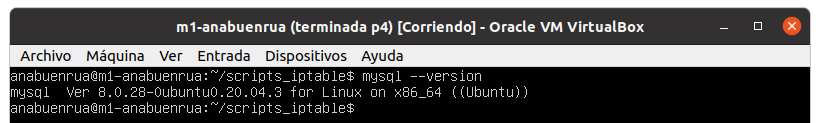
\includegraphics[scale=0.5]{mysql_1}
\end{center}
\end{figure}

Ahora vamos a conectarnos al servidor de mysql. No vamos a usar ninguna contraseña por comodidad, así que cuando nos la pide le damos a enter.

A continuación creamos la base de datos 'estudiante' y le decimos que la use. Una vez la tenemos seleccionada creamos la tabla 'datos', que va a contener campos para el nombre, apellidos, usuario y correo de cada estudiante.

Finalmente añado mis datos a la tabla insertando una tupla, siendo estos Ana Buendía Ruiz-Azuaga, con usuario anabuenrua y correo anabuenrua@correo.ugr.es. Este procedimiento puede verse en \eqref{mysql_2}

\begin{figure}[h!]
\begin{center}
\caption{Creación de la base de datos estudiante y su tabla datos, insertando una tupla.}
\label{mysql_2}
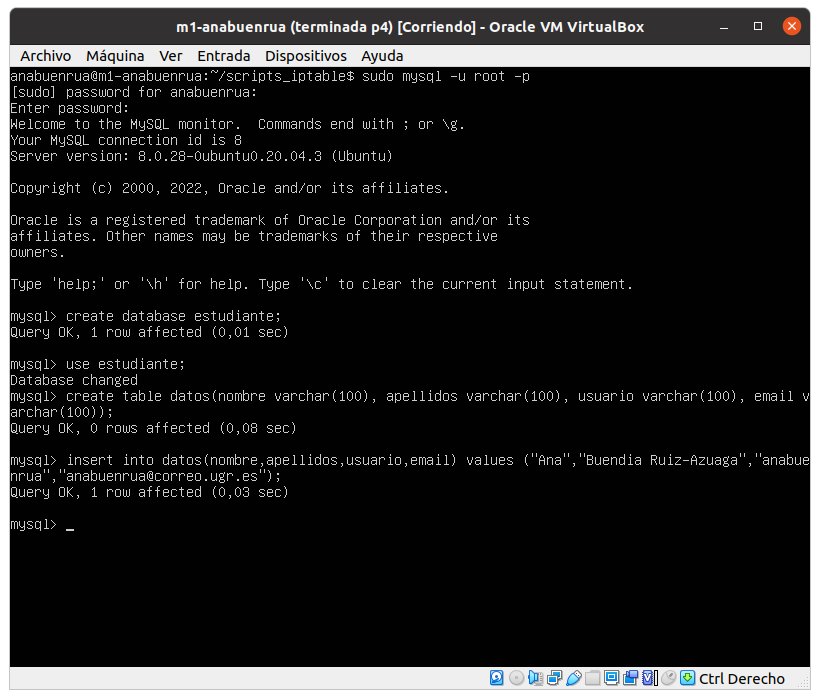
\includegraphics[scale=0.5]{mysql_2}
\end{center}
\end{figure}


\section{Opciones avanzadas}

Como opciones avanzadas, a la hora de crear las tablas podemos especificar que ciertos campos sean no nulos, sean únicos o que se usen como clave primaria (deben ser no nulos y únicos).

Para ello se usan las palabras clave \verb|NOT NULL|, \verb|UNIQUE| y \verb|PRIMARY KEY|. Un ejemplo de uso en una tabla de ejemplo sería:

\begin{verbatim}
CREATE TABLE tasks (
    id INT AUTO_INCREMENT PRIMARY KEY,
    title VARCHAR(255) UNIQUE,
    start_date DATE NOT NULL,
    end_date DATE
);
\end{verbatim}

Además, al insertar nuevas tuplas no hace falta indicar los campos de la tabla donde se va a insertar el valor mientras los valores se especifiquen en el mismo orden de definición de los campos. Aún así, esto puede traer problemas porque si tenemos scripts para introducir las tuplas y cambiamos la estructura de la tabla, también habría que reescribir todos los scripts para insertar las tuplas. Por ello no suele usarse.

También, para consultar información sobre las tablas podemos usar \verb|SELECT| para ver su contenido o |DESCRIBE|, como se ve en \eqref{mysql_3}.

\begin{figure}[h!]
\begin{center}
\caption{Uso de SELECT y DESCRIBE para consultar información de la tabla datos.}
\label{mysql_3}
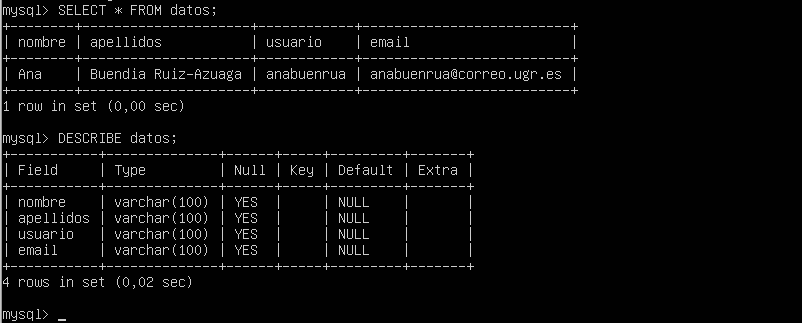
\includegraphics[scale=0.5]{mysql_3}
\end{center}
\end{figure}

\chapter{Mysqldump}

A continuación vamos a replicar la base de datos estudiante de m1 en m2 usando \verb|mysqldump|.

Comenzamos bloqueando las tablas para que sean de solo lectura, y así asegurarnos de que no se modifican mientras se realiza la copia. Se puede ver en \eqref{dump_1}.

\begin{figure}[h!]
\begin{center}
\caption{Establecemos bloqueo en las tablas para que solo se permita lectura.}
\label{dump_1}
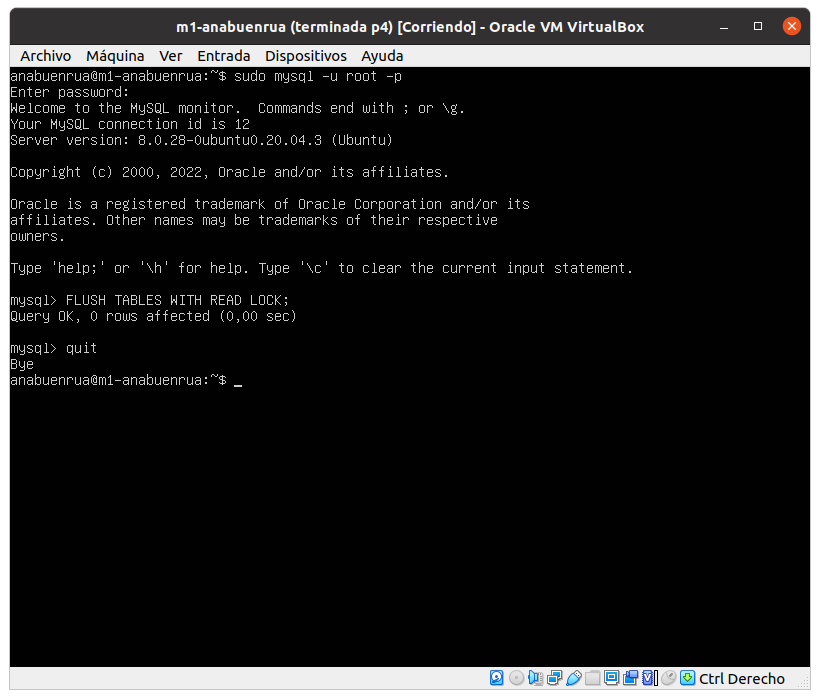
\includegraphics[scale=0.5]{dump_1}
\end{center}
\end{figure}

Copiamos la base de datos en un archivo \verb|/tmp/estudiante.sql| con \verb|mysqldump| y, una vez terminado, eliminamos el bloqueo a las tablas que habíamos puesto antes, como se muestra en \eqref{dump_2}.

\begin{figure}[h!]
\begin{center}
\caption{Volcado de la base de datos y desbloqueo de las tablas.}
\label{dump_2}
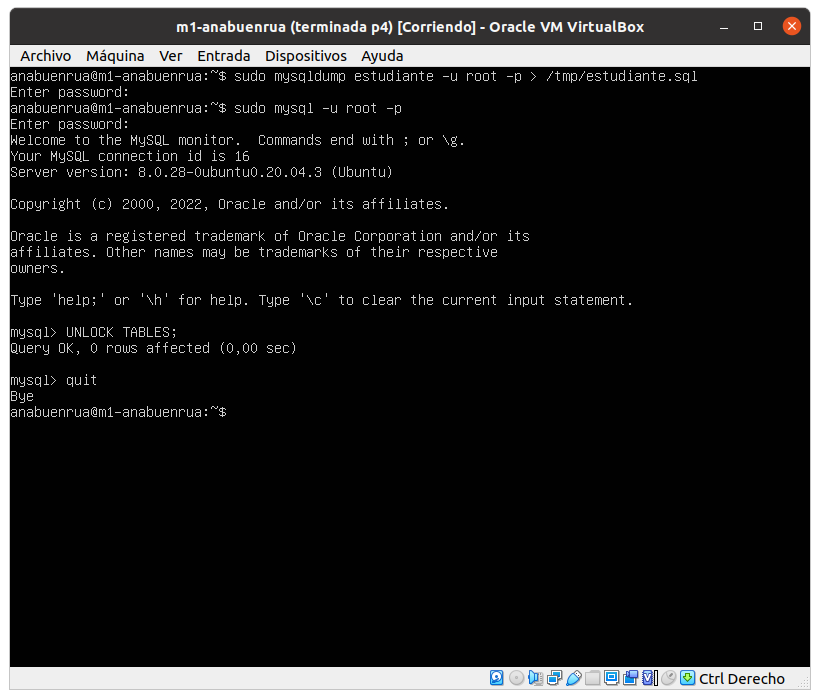
\includegraphics[scale=0.5]{dump_2}
\end{center}
\end{figure}

Ahora copiamos el fichero generado en m1 a m2 mediante scp. \eqref{dump_3}.

\begin{figure}[h!]
\begin{center}
\caption{Copia de /tmp/estudiante.sql de m1 a m2}
\label{dump_3}
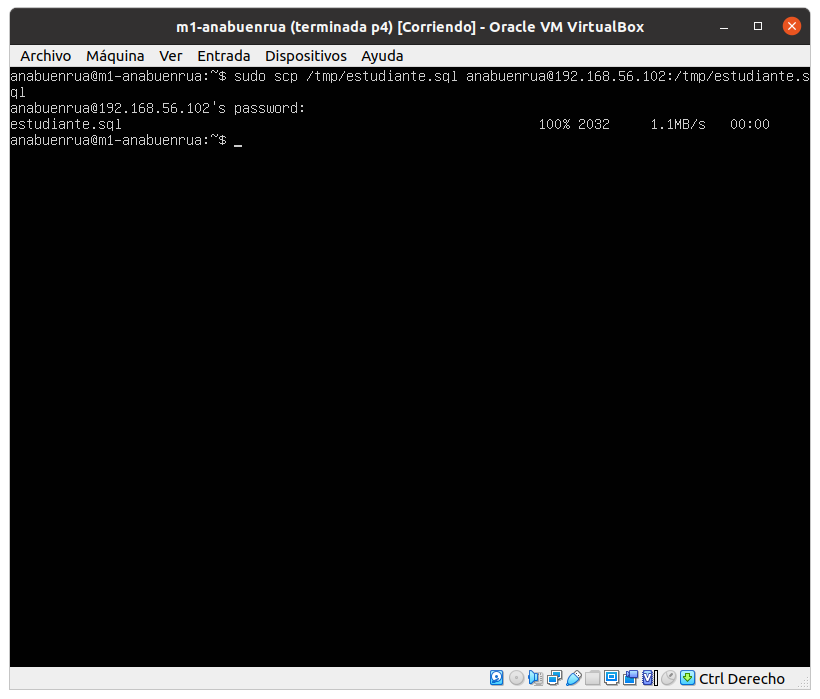
\includegraphics[scale=0.5]{dump_3}
\end{center}
\end{figure}

Finalmente replicamos la base de datos en m2 primero creando la base de datos en sí y luego restaurando los datos de esta usando el fichero que hemos copiado de m1, como se ve en \eqref{dump_4}.

\begin{figure}[h!]
\begin{center}
\caption{Restauramos la base de datos en m2.}
\label{dump_4}
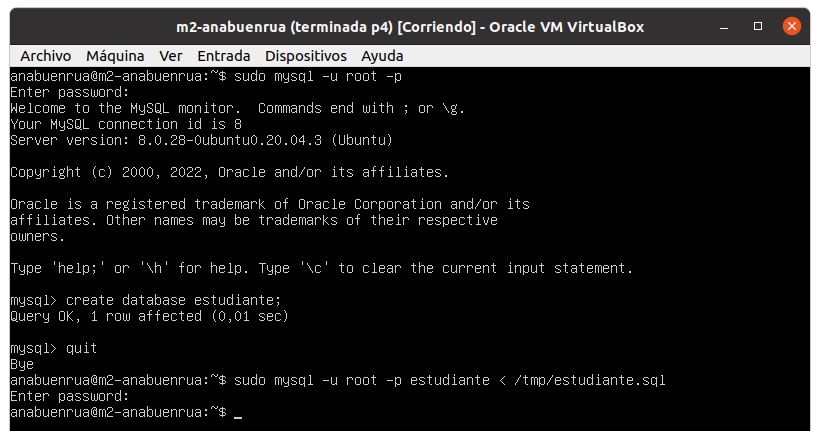
\includegraphics[scale=0.5]{dump_4}
\end{center}
\end{figure}

Ya podemos comprobar que la base de datos se ha copiado correctamente.


\section{Opciones avanzadas}

\verb|mysqldump| tiene varias opciones para ahorrarnos trabajo y asegurarnos de que no cometemos errores importantes como no bloquear las tablas mientras las copiamos, dejarnos bases de datos de interés sin copiar o similares.

De entre esas opciones destacan \verb|--all-databases|, que sirve para copiar todas las bases de datos. Si solo queremos algunas, podemos usar \verb|--databases <db1> <db2> ...|. 

Otra opción interesante es \verb|--add-drop-table|, que añade un drop table antes de la creación de cualquier tabla. Así, antes de crear cualquier tabla, si existía previamente en la base de datos primero la borra y luego la crea.

\verb|--lock-tables| bloquea todas las tablas mientras se realiza la copia, evitando así que tengamos que bloquearlas a mano como hemos hecho nosotros.

Finalmente, para obtener información del proceso podemos usar \verb|-v|, que activa el modo verboso.

El uso de algunas de estas opciones avanzadas puede verse en \eqref{dump_5}.

\begin{figure}[h!]
\begin{center}
\caption{Opciones avanzadas de mysqldump.}
\label{dump_5}
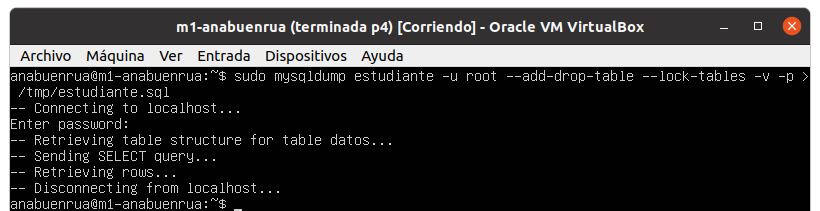
\includegraphics[scale=0.5]{dump_5}
\end{center}
\end{figure}

\chapter{Configuración maestro-esclavo}

Para aplicar una configuración maestro-esclavo lo primero es editar el fichero

\verb|/etc/mysql/mysql.conf.d/mysqld.cnf| en m1 como se muestra, comentando la línea de \verb|bind-address|, especificando los ficheros de log de error y de bin y poniendo el \verb|server-id| a 1. El fichero queda como se muestra en \eqref{esclavo_1}.

\begin{figure}[h!]
\begin{center}
\caption{Fichero /etc/mysql/mysql.conf.d/mysqld.cnf.}
\label{esclavo_1}
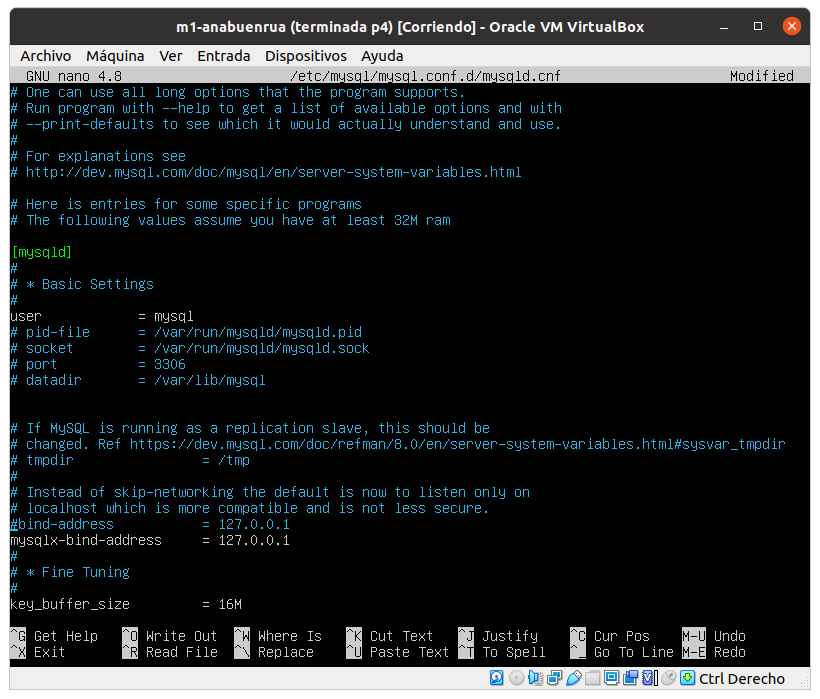
\includegraphics[scale=0.5]{esclavo_1}
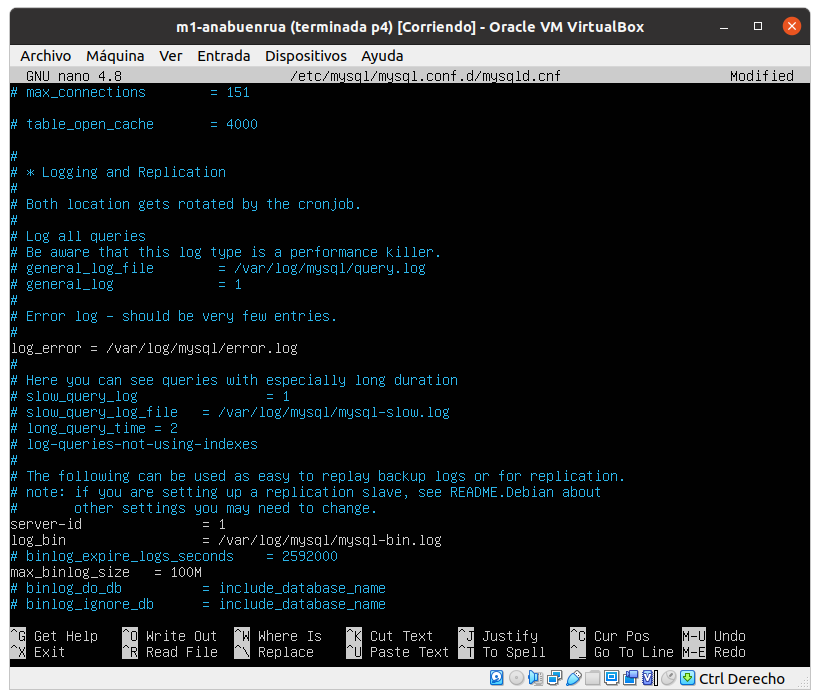
\includegraphics[scale=0.5]{esclavo_2}
\end{center}
\end{figure}

Reiniciamos el servicio con \verb|sudo systemctl restart mysql| y comprobamos que ha ido bien con \verb|sudo systemctl status mysql|.

Ahora en m2 editamos el fichero \verb|/etc/mysql/mysql.conf.d/mysqld.cnf| igual que en m1, pero poniendo su \verb|server-id| a 2, y de nuevo reiniciamos el servicio como antes.

Volviendo a m1, vamos a crear un usuario esclavo. Para crear el usuario correctamente, nos fijamos en la versión de mysql que se comprobó al principio, siendo esta la 8.0.28.

Por tanto, en mysql ejecutamos las órdenes de \eqref{esclavo_3}.

\begin{figure}[h!]
\begin{center}
\caption{Creación del usuario esclavo, dándole privilegios y bloqueando las tablas.}
\label{esclavo_3}
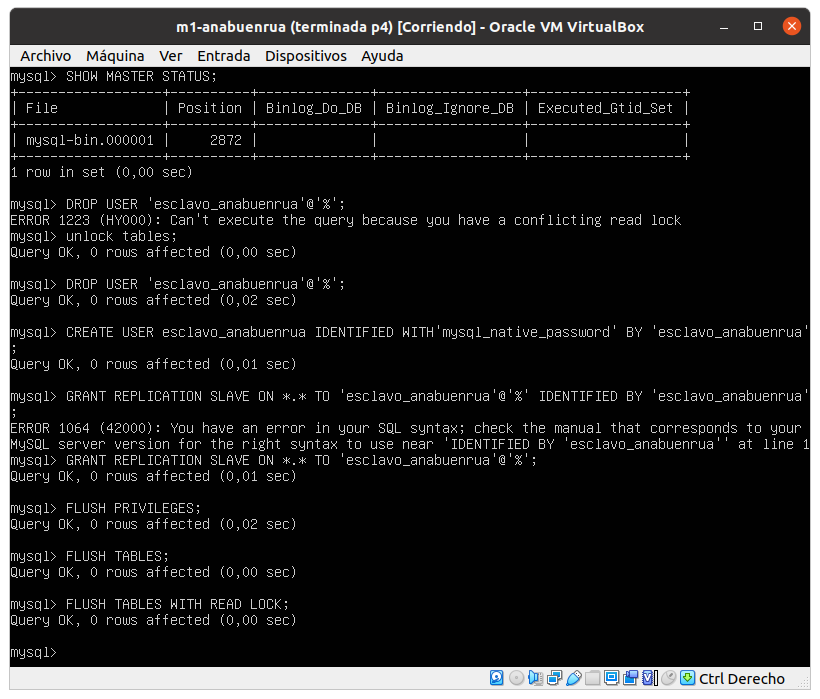
\includegraphics[scale=0.5]{esclavo_3a}
\end{center}
\end{figure}

En \eqref{esclavo_3} observamos que si intentamos otorgar privilegios como indica el guión con \verb|IDENTIFIED BY| da error. Al consultar la documentación vemos que en la versión de mysql que estamos usando no se debe indicar esta opción, así que repetimos la orden omitiendo esta parte y ya funciona sin problemas.

También es destacable que al crear el usuario en \eqref{esclavo_3} usamos

\verb|IDENTIFIED WITH'mysql_native_password'|, esto se debe a que realicé la configuración primeramente sin especificar esta opción, y por defecto se usa ssl con sha256, provocando que al intentar conectarse desde el esclavo ocurriera un error porque la conexión no era segura. El error que ocurría se muestra en \eqref{esclavo_error}. La solución de especificar esta opción la he obtenido de \href{https://stdworkflow.com/927/2061-authentication-plugin-caching-sha2-password-reported-error-authentication-require-secure-connection)}{aquí}.

\begin{figure}[h!]
\begin{center}
\caption{Error al configurar maestro-esclavo al no especificar mysql\_native\_password}
\label{esclavo_error}
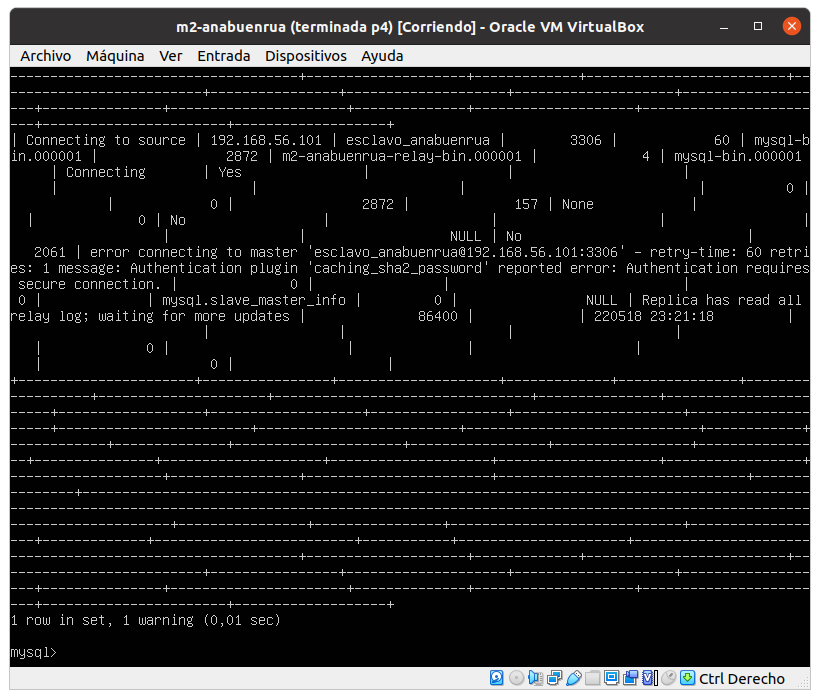
\includegraphics[scale=0.5]{ERROR}
\end{center}
\end{figure}

Ahora mostramos el estado del maestro en \eqref{esclavo_4}, obteniendo así la información necesaria para configurar m2 después.

\begin{figure}[h!]
\begin{center}
\caption{Estado del maestro.}
\label{esclavo_4}
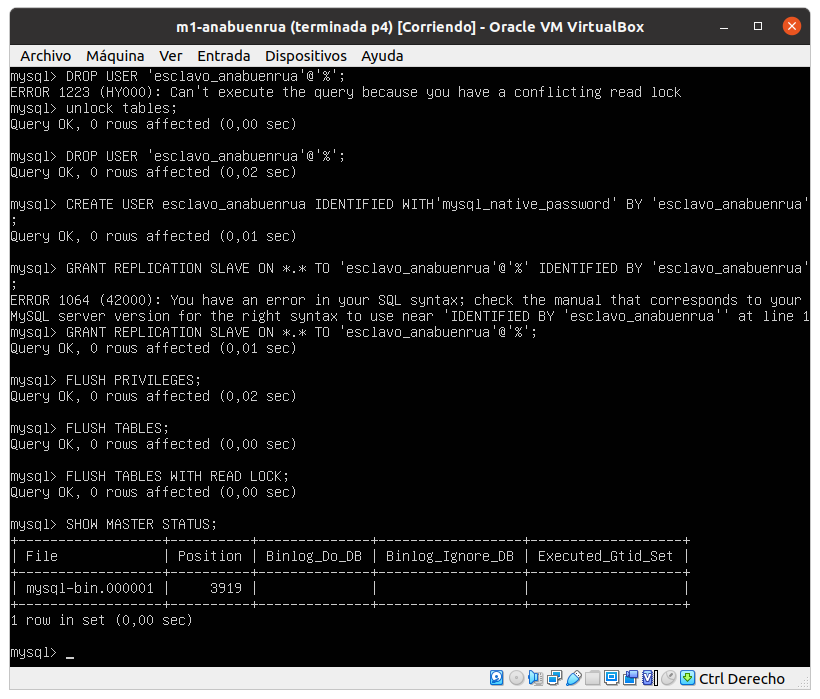
\includegraphics[scale=0.5]{esclavo_4a}
\end{center}
\end{figure}

Ahora con esta información configuramos en m2 los datos del maestro como se muestra en \eqref{esclavo_5}.

\begin{figure}[h!]
\begin{center}
\caption{Configuración de los datos del maestro en m2.}
\label{esclavo_5}
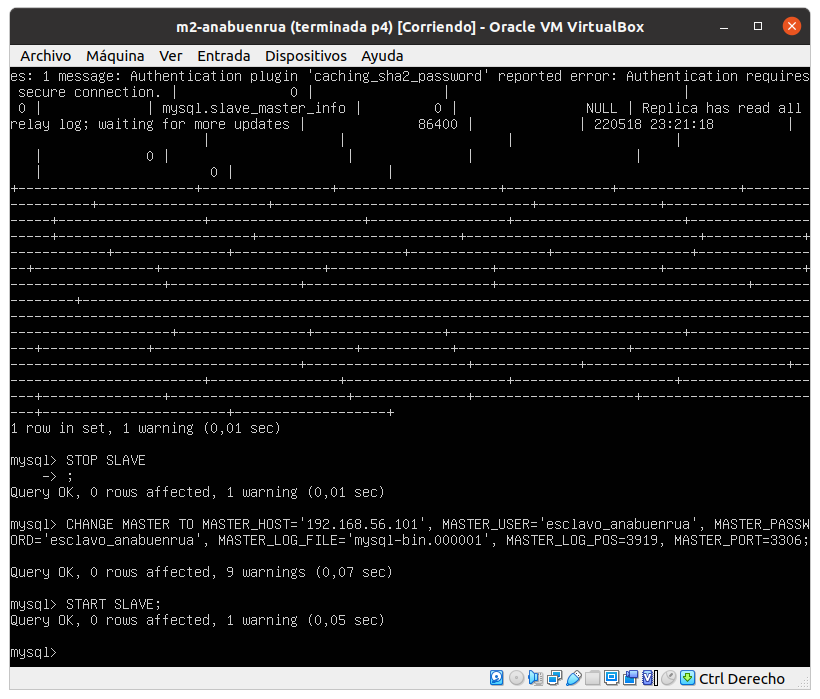
\includegraphics[scale=0.5]{esclavo_5a}
\end{center}
\end{figure}

Finalmente quitamos el bloqueo de las tablas en m1 como se ve en \eqref{esclavo_6} y comprobamos el estado del esclavo \eqref{esclavo_8}.

\begin{figure}[h!]
\begin{center}
\caption{Desbloqueo de las tablas en m1 tras configurar m2.}
\label{esclavo_6}
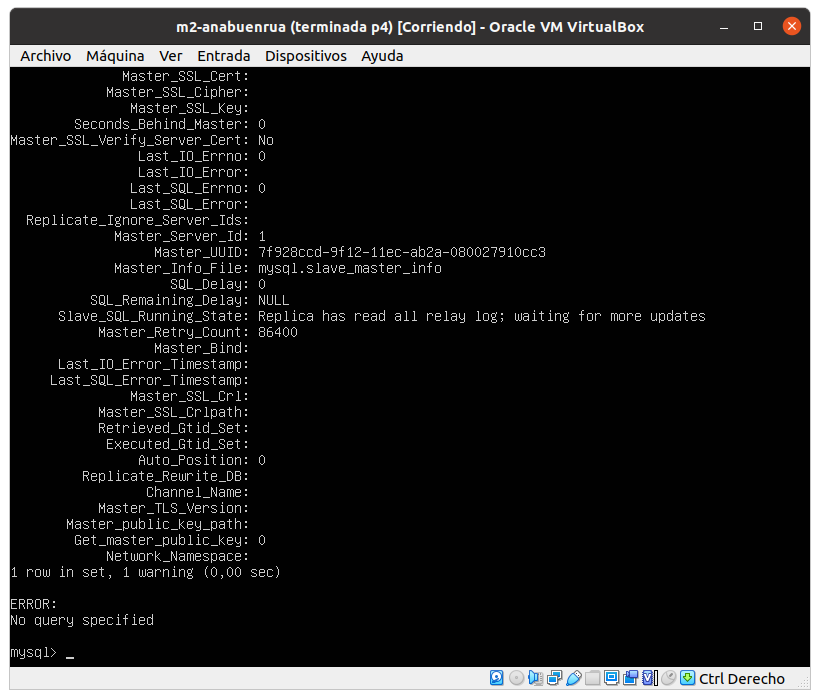
\includegraphics[scale=0.5]{esclavo_8a}
\end{center}
\end{figure}

\begin{figure}[h!]
\begin{center}
\caption{Estado del esclavo.}
\label{esclavo_8}
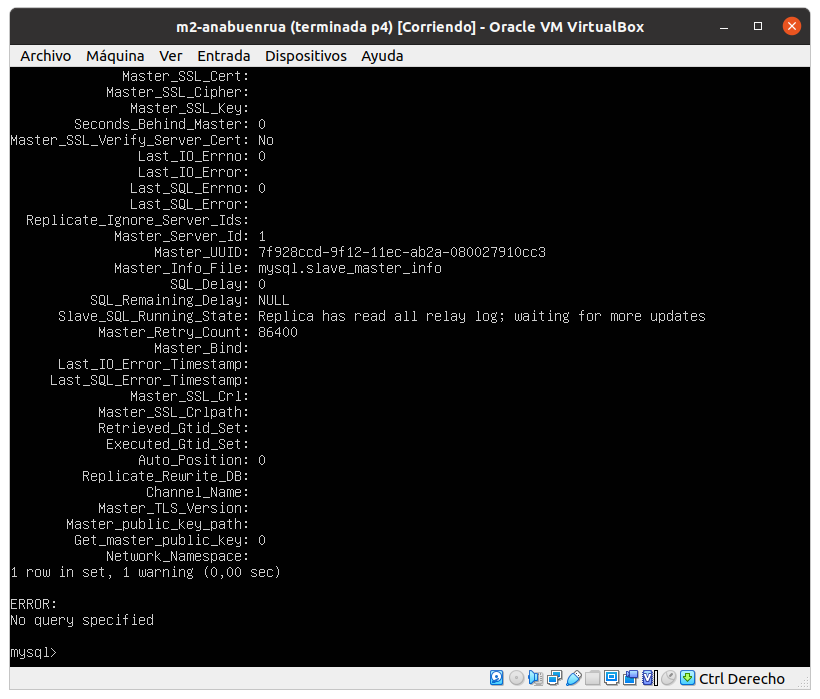
\includegraphics[scale=0.5]{esclavo_6a}
\end{center}
\end{figure}

Parece que funciona porque en \eqref{esclavo_8} el parámetro \verb|Seconds_Behind_Master| tiene valor 0.

Finalmente nos aseguramos de que todo funciona correctamente, pues si insertamos un usuario 'prueba' en m1, vemos que aparece en m2, como se ve en \eqref{esclavo_9}

\begin{figure}[h!]
\begin{center}
\caption{Insertamos tupla de prueba en m1 y comprobamos que los cambios se reflejan en m2.}
\label{esclavo_9}
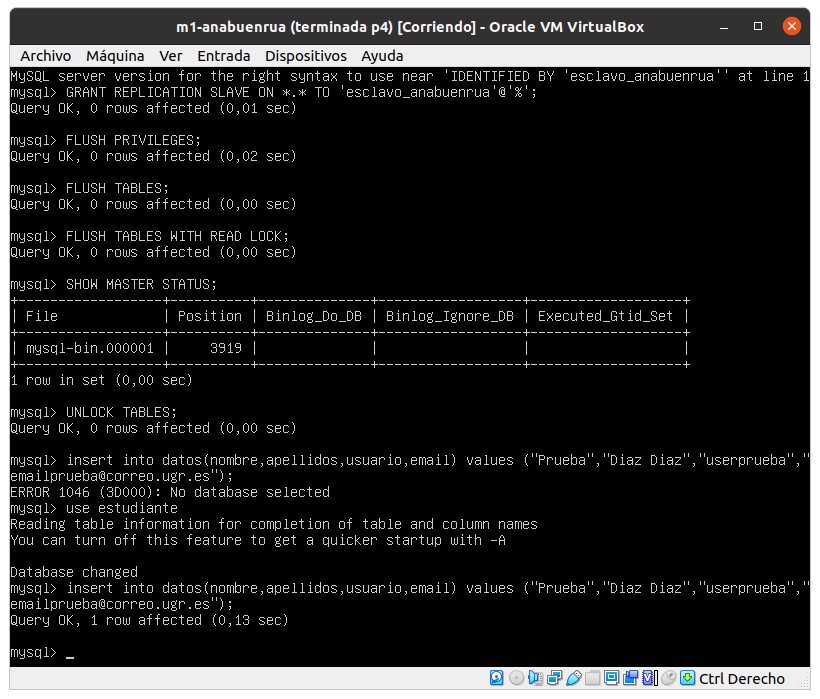
\includegraphics[scale=0.5]{esclavo_9}
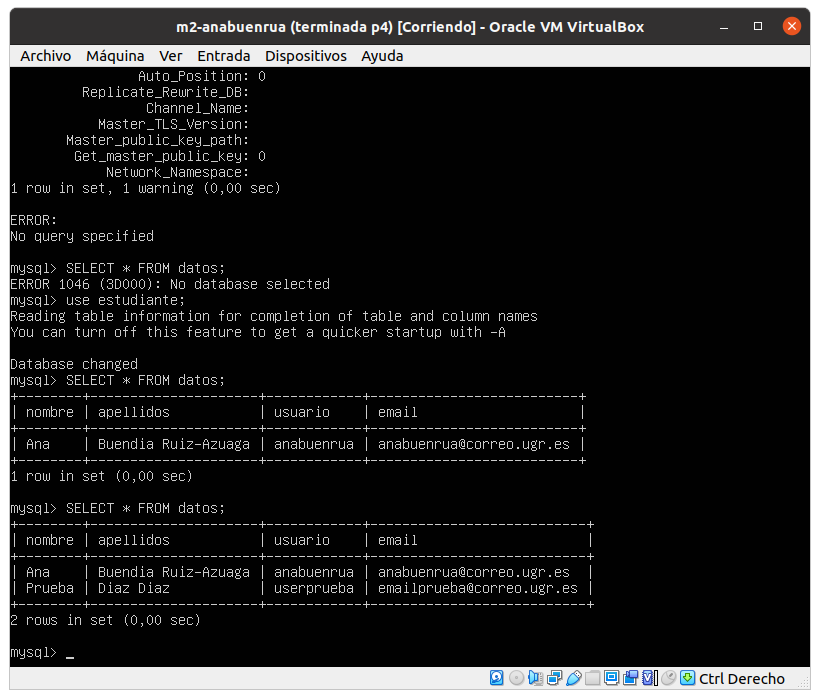
\includegraphics[scale=0.5]{esclavo_10}
\end{center}
\end{figure}



\chapter{Mostrar estado de los servidores}

El estado del maestro puede verse en \eqref{esclavo_4} y el del esclavo en \eqref{esclavo_8}. Vamos a interpretar brevemente lo que nos están indicando estos estados.

El estado del maestro nos muestra información necesaria para la configuración del esclavo.

Por otra parte, el tener un valor $0$ en \verb|Seconds_Behind_Master| en el estado del esclavo, quiere decir que la base de datos de la máquina esclava lleva 0 segundos de retraso en procesar los binary-log que se han especificado.

Que sea 0 suele significar que el esclavo está al día con el maestro, mientras que si tiene un valor mayor es que aún está procesando.

Además, en el estado del esclavo \eqref{esclavo_8} pueden verse los errores obtenidos. En \eqref{esclavo_8} no se muestra ningún error ya que la configuración ha resultado correctamente, pero en \eqref{esclavo_error} podemos ver un error al no poder conectarnos por SSL, como ya se ha comentado antes. Los errores de la configuración se muestran en las líneas de error LAST\_IO\_ERROR y LAST\_SQL\_ERROR muestra los error de SQL.

\chapter{Configuración maestro-maestro}

Para realizar la configuración maestro-maestro vamos a repetir la configuración que ya hemos hecho de maestro-esclavo, pero esta vez tomando como maestro a m2 y como esclavo a m1, esto es, inviertiendo los roles de antes.

De esta forma, ambas máquinas son maestras y esclavas a la vez, obteniendo así la configuración maestro-maestro.

Como el archivo \verb|/etc/mysql/mysql.conf.d/mysqld.cnf| ya está editado, comenzamos creando el usuario esclavo en m2 como se muestra en \eqref{maestro_1}.

\begin{figure}[h!]
\begin{center}
\caption{Creación del usuario esclavo en m2 otorgándole privilegios y bloqueo de las tablas.}
\label{maestro_1}
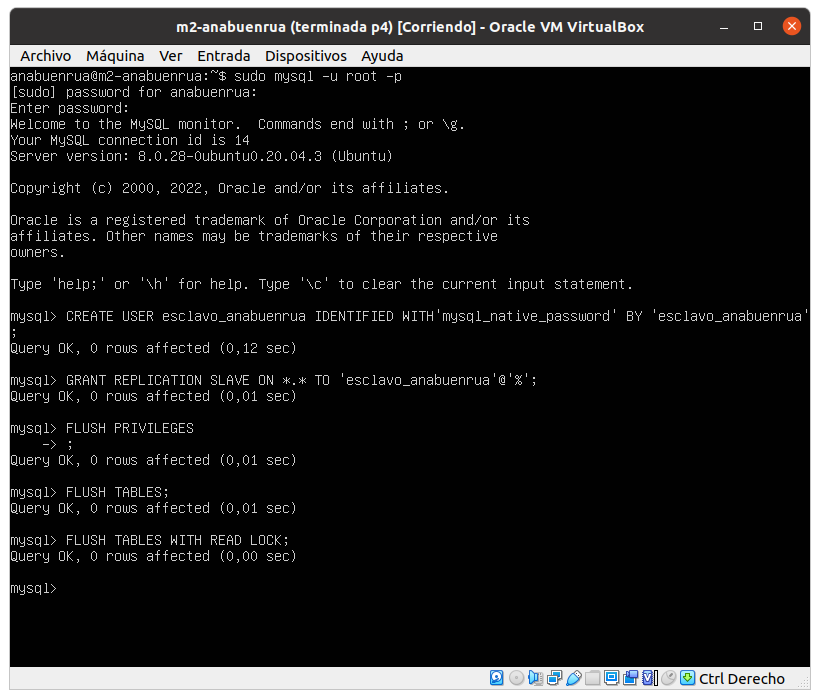
\includegraphics[scale=0.5]{maestro_1}
\end{center}
\end{figure}

Ahora mostramos el estado del maestro en \eqref{maestro_2}.

\begin{figure}[h!]
\begin{center}
\caption{Estado del maestro.}
\label{maestro_2}
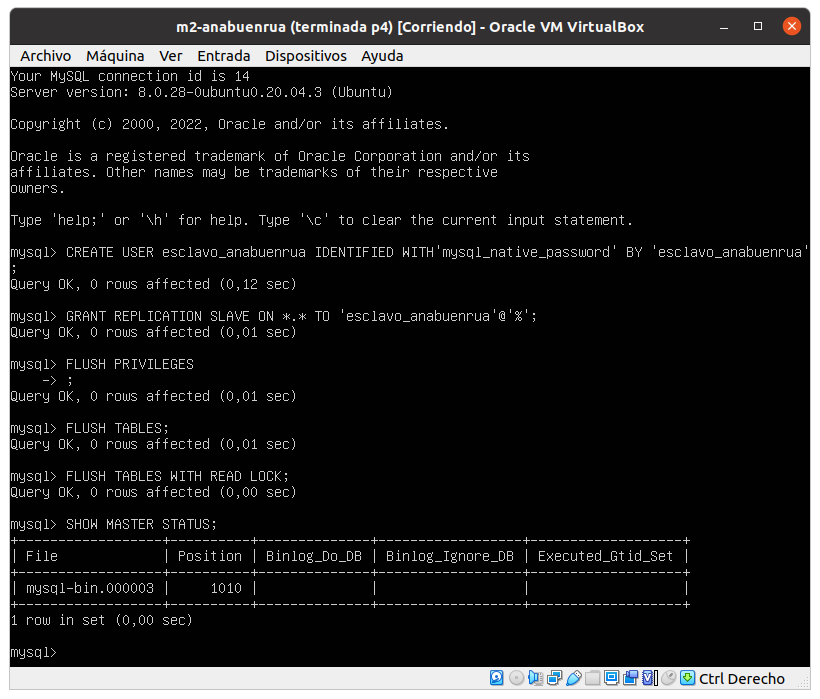
\includegraphics[scale=0.5]{maestro_2}
\end{center}
\end{figure}

Ahora en m1 configuramos el esclavo con los datos del maestro y lanzamos el esclavo, como se ve en \eqref{maestro_3}.

\begin{figure}[h!]
\begin{center}
\caption{Configuración de los datos del maestro en m1.}
\label{maestro_3}
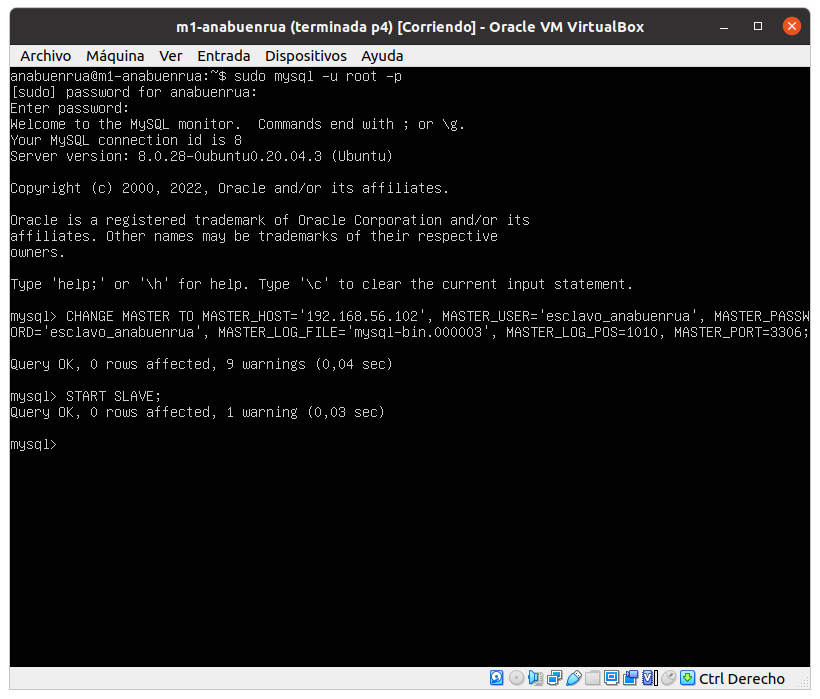
\includegraphics[scale=0.5]{maestro_3}
\end{center}
\end{figure}

Finalmente eliminamos el bloqueo se las tablas en \eqref{maestro_4} y comprobamos el estado del esclavo en \eqref{maestro_5}.

\begin{figure}[h!]
\begin{center}
\caption{Desbloqueo de las tablas en m2.}
\label{maestro_4}
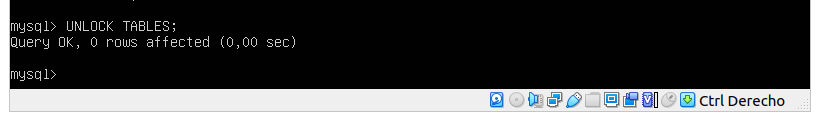
\includegraphics[scale=0.5]{maestro_4}
\end{center}
\end{figure}

\begin{figure}[h!]
\begin{center}
\caption{Estado del esclavo.}
\label{maestro_5}
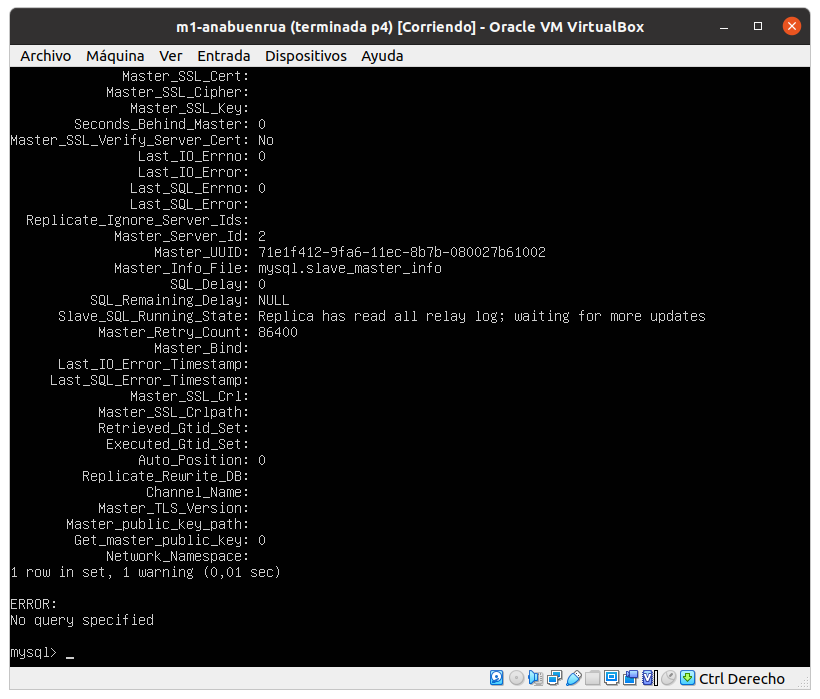
\includegraphics[scale=0.5]{maestro_5}
\end{center}
\end{figure}

Comprobamos que si introducimos en datos una fila desde m1 (nombre PruebaM1) se actualiza en m2 y que pasa lo mismo si desde m2 introducimos una fila (nombre PruebaM2), como se muestra en \eqref{maestro_6}.

\begin{figure}[h!]
\begin{center}
\caption{Comprobación del correcto funcionamiento de la configuración maestro-maestro.}
\label{maestro_6}
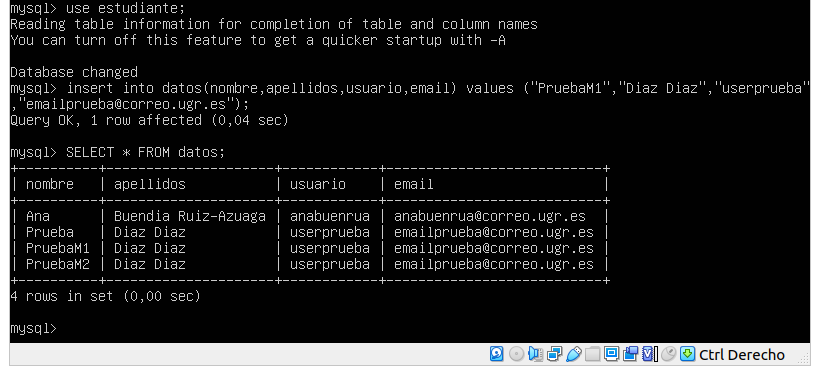
\includegraphics[scale=0.5]{maestro_8}
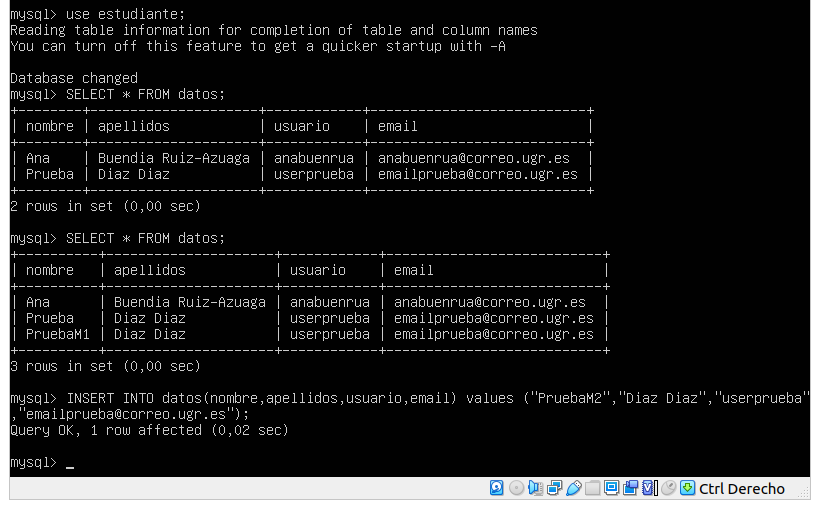
\includegraphics[scale=0.5]{maestro_9}
\end{center}
\end{figure}


\chapter{Configuración de IPTABLES}

Ya hemos terminado de configurar la replicación de base de datos, pero todas las pruebas y conexiones se han realizado con todas las reglas de iptables que hicimos en la práctica anterior sin aplicar, es decir, se aceptaba todo el tráfico.

Con el fin de proteger nuestra granja web, vamos a añadir reglas para abrir las conexiones de mysql (por el puerto 3306) solamente entre m1 y m2, de forma que toda la granja esté protegida como antes y se pueda realizar la replicación de bases de datos sin desactivar las reglas.

Para ello, editamos el archivo \verb|/home/anabuenrua/configuracion_avanzada.sh| en m1 y m2. Por ejemplo el fichero de m1 se muestra en \eqref{iptables_1}, para m2 bastaría cambiar la IP especificada.

\begin{figure}[h!]
\begin{center}
\caption{Fichero /home/anabuenrua/scripts\_iptable/config\_avanzada.sh para permitir tráfico por el puerto 3306 solo entre m1 a m2 de m1.}
\label{iptables_1}
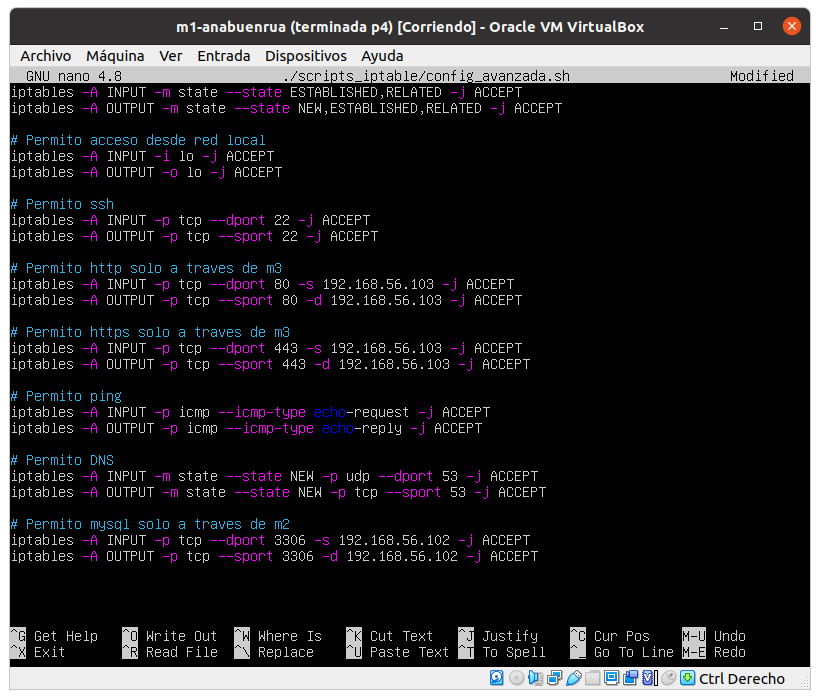
\includegraphics[scale=0.5]{iptables_1}
\end{center}
\end{figure}

Comprobamos que funciona adecuadamente y hacemos las reglas persistentes como se indicaba en la práctica anterior, como podemos ver en \eqref{iptables_2}.

\begin{figure}[h!]
\begin{center}
\caption{Hacemos las reglas persistentes.}
\label{iptables_2}
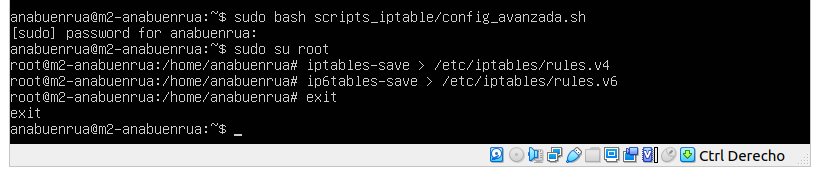
\includegraphics[scale=0.5]{iptables_3}
\end{center}
\end{figure}



%\input{chapters/capitulo_1}


% Part II
%\input{chapters/chapter5}

% ----------------------- %
% BIBLIOGRAFÍA
% ----------------------- %

% Estilo de cita.
%\usepackage{natbib} YA SE IMPORTA EN OTRO PUNTO, NO HACE FALTA PONERLO AQUI
% FUENTE CUSTOM
%\bibliographystyle{apa-good}
% formato de citas original
\bibliographystyle{unsrtnat}

%[citestyle=numeric]

% Añadimos la bibliografía al índice
%\phantomsection
%\addcontentsline{toc}{chapter}{Bibliografía}


\chapter{Bibliografía}
\begin{itemize}
\item Diapositivas y guión de la práctica.
\item \href{http://nginx.org/en/docs/}{http://nginx.org/en/docs/}
\item \href{https://www.digitalocean.com/community/tutorials/how-to-create-a-self-signed-ssl-certificate-for-apache-in-ubuntu-18-04-es}{https://www.digitalocean.com/community/tutorials/how-to-create-a-self-signed-ssl-certificate-for-apache-in-ubuntu-18-04-es}
\item \href{https://linuxconfig.org/how-to-make-iptables-rules-persistent-after-reboot-on-linux}{https://linuxconfig.org/how-to-make-iptables-rules-persistent-after-reboot-on-linux}
\item \href{https://www.hostinger.com/tutorials/iptables-tutorial}{https://www.hostinger.com/tutorials/iptables-tutorial}
\item \href{https://www.codegrepper.com/code-examples/shell/install+certbot+ubuntu+20.04}{https://www.codegrepper.com/code-examples/shell/install+certbot+ubuntu+20.04}
\item \href{https://www.cyberciti.biz/faq/unix-linux-check-if-port-is-in-use-command/}{https://www.cyberciti.biz/faq/unix-linux-check-if-port-is-in-use-command/}
\item \href{https://easyengine.io/tutorials/nginx/troubleshooting/emerg-bind-failed-98-address-already-in-use/}{https://easyengine.io/tutorials/nginx/troubleshooting/emerg-bind-failed-98-address-already-in-use/}

\end{itemize}

%\bibliography{bib/library}

\end{document}